\section{Prehľad problematiky}
Digitalizácia najrôznejších aspektov nášho života je prirodzeným prejavom technologického pokroku. Vďaka tomu sa 
pojmy, ako zmiešaná realita, rozšírená realita či virtuálna realita v~priebehu posledných dekád začali stávať neoddeliteľnou súčasťou nášho jazyka. 
Na to, aby sme lepšie porozumeli tomu, čo to zmiešaná realita vlastne je, pokladáme za nevyhnutné venovať niekoľko odstavcov aj zvyšným dvom pojmom.

\subsection{Virtuálna realita}
\begin{quote}\itshape
  The ultimate display would, of course, be a room within which the computer can control the existence of matter. A chair displayed in such a~room 
  would be good enough to sit in. Handcuffs displayed in such a room would be confining, and a~bullet displayed in such a~room would be fatal. 
  With appropriate programming such a display could literally be the Wonderland into which Alice walked.
\end{quote}
Týmito slovami v roku 1965 Ivan Sutherland vo svojom článku \cite{sutherlandUltimateDisplay1965b} sformuloval ideu, ktorá predstavuje raný popis 
imerzívneho\footnote{Z angl. \emph{immersive} - voľne preložené ako vťahujúci do deja} displeja v dobe, keď vtedajšie zariadenia bežne umožňovali 
zobrazovať rovné čiary, uvažovalo sa, že zobrazovanie kriviek by mohlo byť užitočné a žiadna komerčne dostupná obrazovka nebola schopná vykresliť farbou 
vyplnenú plochu \cite{sutherlandUltimateDisplay1965b}. 

Krátko potom Sutherland skonštruoval prvý interaktívny systém slúžiaci na zobrazovanie virtuálnej reality, ktorý si vyslúžil priliehavú prezývku 
\emph{Damoklov meč} \cite[5]{schmalstiegAugmentedRealityPrinciples2016}, pozri obr. \ref{sutherland-device}. Trojrozmerný displej s~upevnením na hlavu, ktorý 
Sutherland vo svojej práci \cite{sutherlandHeadmountedThreeDimensional1968} popísal v~roku 1968, pozostával zo špeciálnych okuliarov, 
ktoré na sebe mali upevnené dve miniatúrne obrazovky typu \acrshort{crt} a~boli pevnou súčasťou ramena visiaceho zo stropu miestnosti. 
Okrem zníženia fyzickej záťaže používateľa, ktorá vznikala kvôli hmotnosti zariadenia, toto rameno slúžilo ako mechanický snímač polohy hlavy a~spolu s~ďalším, 
ultrazvukovým snímačom generovalo vstupné údaje pre výpočet rotačnej a~translačnej matice. Tie boli súčasťou operácií nevyhnutných pre dynamické generovanie obrazu. 
Objekty, z~ktorých pozostával výsledný obraz, boli poskladané z~jednoduchých čiar a~vytvárali tzv.~wireframe model.

\begin{figure}[!htbp]
  \centering
  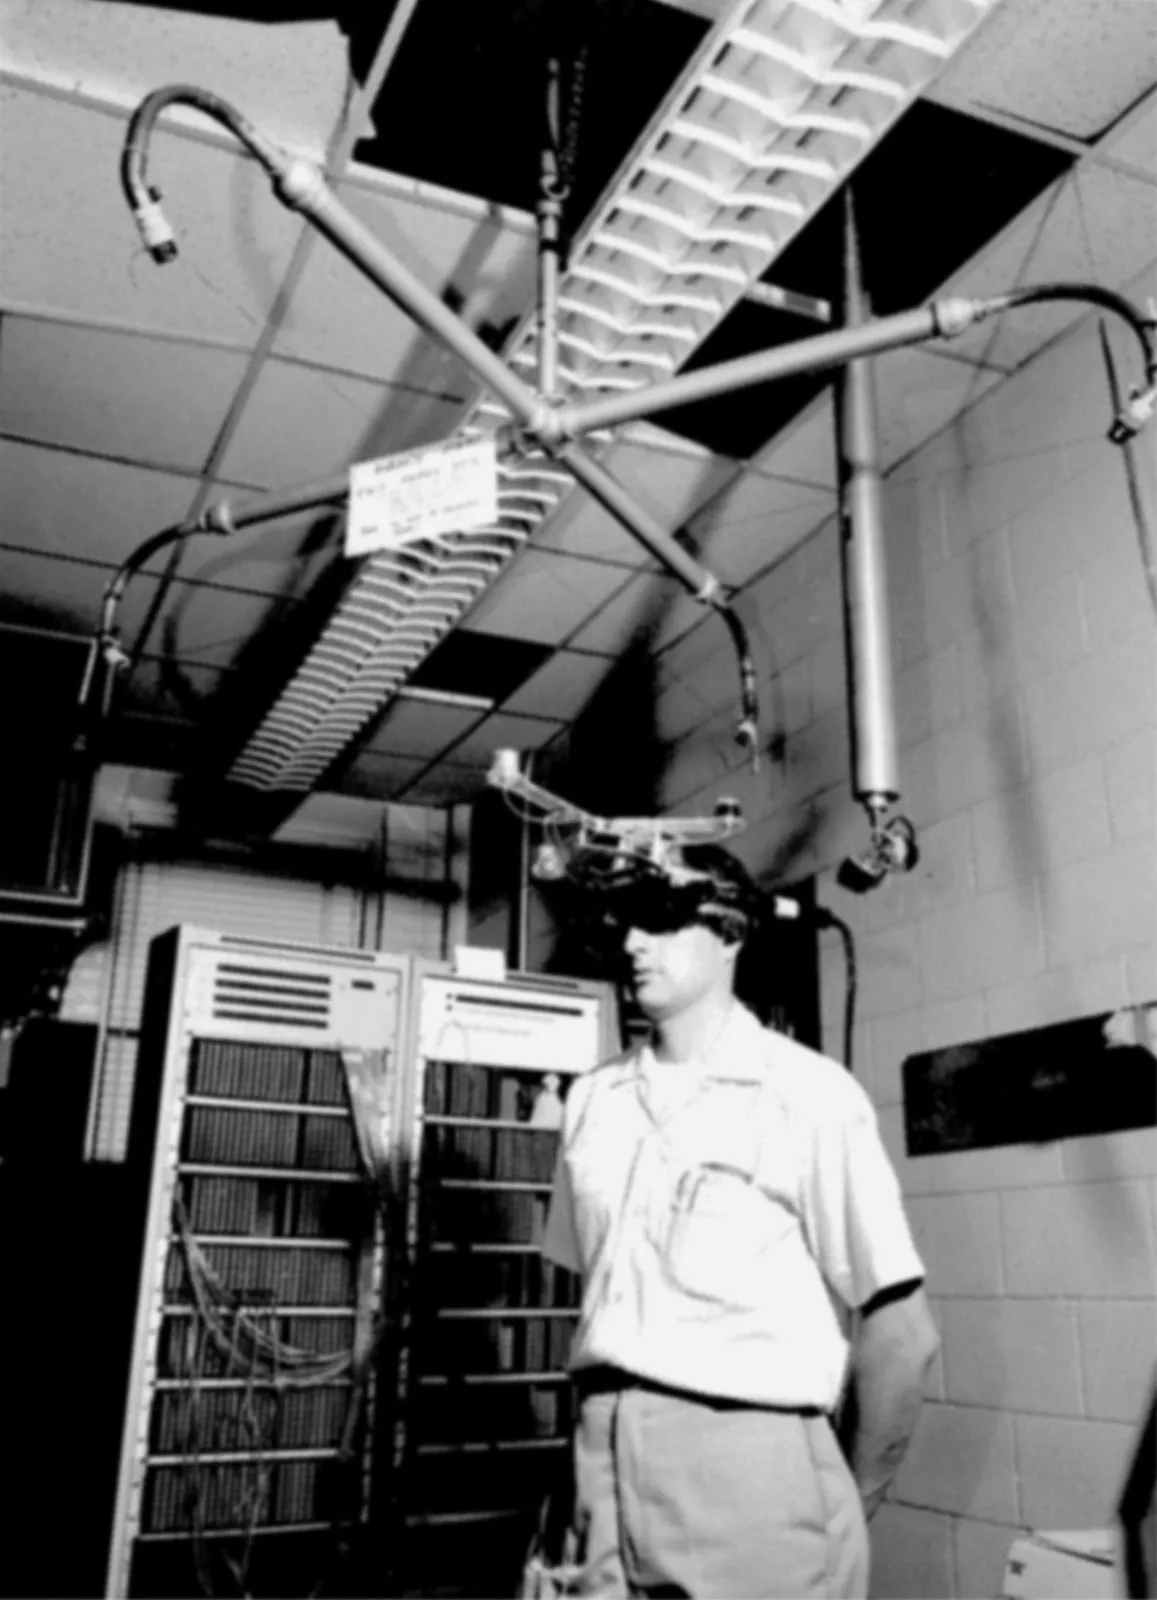
\includegraphics[width=7cm]{img/display-device-Ivan-Sutherland-Harvard-University-1967.jpg}
  \caption{Zobrazovacie zariadenie Ivana Sutherlanda}
  \label{sutherland-device}
\end{figure}	

Sutherlandovo dielo významne prispelo k rozvoju myšlienok a technológií súvisiacimi s~vizualizáciou umelého sveta. Postupom času vzniklo množstvo ďalších 
prototypov rôznorodých systémov, ktoré sa líšili nie len účelom použitia, ale aj spôsobom vzájomnej interakcie s~človekom a~aj tým, či a~ako veľmi bol umelý 
svet prepojený s tým skutočným. Ako príklad uvedieme systém VIDEOPLACE Myrona Kruegera z roku 1985, ktorý kombinuje zosnímanú postavu používateľa s~umelo vytvoreným 
prostredím. Krueger navrhuje využitie tohto systému pre účely telekomunikácie uvádzajúc, že komunikácia medzi priateľmi či obchodnými partnermi nie je 
obmedzená len slovami, a teda je jednoznačne žiadúce, aby geograficky vzdialené osoby mohli zdieľať spoločné virtuálne prostredie 
\cite{kruegerVIDEOPLACEArtificialReality1985}.

Práve Kruegerov systém sprostredkúva to, čo v súčasnej terminológii môžeme označiť ako virtuálnu realitu. Tá prenesie človeka do úplne odlišného prostredia, 
reálne okolie a objekty v ňom nahradí počítačom generovanými, s~cieľom poskytnúť používateľovi intenzívny zážitok z~nového sveta, akoby sa v~ňom skutočne nachádzal
\cite{brighamRealityCheckBasics2017}. 

V deväťdesiatych rokoch minulého storočia bola snaha o rozšírenie zariadení pre virtuálnu realitu medzi bežných spotrebiteľov. Tieto zariadenia však boli cenovo
nedostupné a~spôsobovali používateľom nevoľnosť. Príčinou nevoľnosti bol nesúlad medzi zrakovým a vestibulárnym vnemom; ten bol spôsobený vysokou latenciou medzi pohybom 
hlavy používateľa a~reakciou VR zariadenia na tento pohyb prekreslením virtuálnej scény. 

Prelom nastal až v roku 2014, keď Palmer Luckey, 
zakladateľ spoločnosti Oculus, objavil spôsob, ako znížiť dobu trvania vyhodnocovania polohy hlavy za použitia gyroskopu, akcelerometra a magnetometra. 
Tento úspech opäť naštartoval záujem o túto technologickú oblasť \cite{brighamRealityCheckBasics2017}. V súčasnosti medzi najrozšírenejšie zariadenia patria Oculus Rift S,
HTC Vive Pro, HTC Vive Cosmos, Valve Index a Samsung HMD Odyssey+ \cite{angelovModernVirtualReality2020}. Ďalšou z možností, ktorú propagujú výrobcovia, ako Samsung, Google
a LG, je použitie smartfónu ako displeja vo VR headsete, čo predstavuje cenovo dostupnú alternatívu. Ako príklad uvádzame Samsung Gear VR, ktorý je kompatibilný
s~akýmkoľvek modelom Samsung Galaxy; ďalší príklad je dnes už nepodporovaný Google Cardboard a Google Daydream. 

\subsection{Rozšírená realita}
Podľa výskumu popísaného v článku \cite{speicherWhatMixedReality2019a} definícia rozšírenej reality nie je ani zďaleka tak jednoznačná, ako v prípade virtuálnej reality. 
Jeho autori položili desiatim osobám, ktoré sa zaoberajú virtuálnou a rozšírenou realitou v komerčnej a akademickej sfére, súbor šestnástich otázok, ktoré boli 
navrhnuté tak, aby odhalili rozdiely vo vnímaní toho, čo je virtuálna, rozšírená a zmiešaná realita. Autori uvádzajú, že respondenti sa nezhodovali pri vymenovávaní
relevantných charakteristík rozšírenej reality. Niektorí za rozšírenú realitu pokladajú aj jednoduchú vrstvu\footnote{pôvodne použitý angl. termín \emph{overlay}} 
s~kontextuálnymi informáciami, zatiaľ čo ostatní explicitne uvádzali interakciu s~reálnym prostredím a prekrývanie skutočných objektov počítačom generovanými 
ako jej súčasť.

Chen a Xue uvádzajú, že typický \acrshort{ar} systém musí spĺňať tri podmienky: musí umožňovať interakciu medzi reálnym a virtuálnym obsahom, dokáže v reálnom čase 
prekrývať reálne objekty virtuálnymi, a musí pracovať v trojrozmernom priestore. Takáto funkcionalita vyžaduje použitie rôznych techník sledovania, zobrazovania a
interakcie \cite{chenRenaissanceAugmentedReality2022}.

Techniky sledovania sú používané na zaznamenávanie a overovanie pozície a orientácie používateľov. Zohrávajú dôležitú úlohu pri zosúladení polohy reálnych a virtuálnych
objektov. Pozíciu a orientáciu je možné zisťovať pomocou metód spracovania obrazu, za použitia rozličných senzorov, či kombináciou oboch spôsobov.

Zobrazovacie techniky spájajú virtuálny obsah a reálne prostredie a zobrazujú oboje naraz. V praxi sa uplatnili tri spôsoby zobrazovania: pomocou ručného zariadenia 
(\emph{handheld display}) - napr. smartfón alebo tablet, pomocou náhlavného zariadenia (\emph{headmounted-display}) a za použitia projekcie na povrch reálneho objektu 
(\emph{projection-based display}).

Interakčné techniky zabezpečujú intuitívne používateľské prostredie a adekvátne reakcie systému. Používateľské vstupy pritom môžu byť vo forme gest, hlasových povelov,
prípadne je možné použiť reálny objekt ako ovládací prvok \cite{chenRenaissanceAugmentedReality2022}.

\newpage Pomerne známym zástupcom zariadení pre rozšírenú realitu je zariadenie od spoločnosti Google s~názvom Google Glass. Zariadenie v~tvare bežných 
okuliarov, dostupné len počas pomerne krátkeho obdobia (2013 - 2015) \cite{brighamRealityCheckBasics2017} dokázalo používateľovi zobrazovat informácie na malom displeji tesne
nad pravým okom. 

\subsection{Zmiešaná realita}
Zmiešaná realita je najmenej preskúmaný typ umelej reality, pretože je spomedzi trojice \acrshort{vr}, \acrshort{ar} a \acrshort{mr} najmladší. Podobne, ako v prípade
rozšírenej reality, ani tu nejestvuje úplna zhoda v definícii. 

Podľa \cite{speicherWhatMixedReality2019a} existuje šesť spôsobov chápania \acrshort{mr}; ich názvy ponechávame v pôvodnom znení:
\begin{itemize}
  \item \emph{Continuum}
  \item \emph{Synonym}
  \item \emph{Collaboration}
  \item \emph{Combination}
  \item \emph{Alignment}
  \item \emph{Strong \acrshort{ar}}
\end{itemize}

\noindent Vymenované spôsoby chápania \acrshort{mr} sú vysvetlené v nasledujúcich podkapitolách.

\subsubsection{Continuum}
\acrshort{mr} je chápané v súlade s RV kontinuom\footnote{Reality-Virtuality Continuum}, ktoré je znázornené na obrázku č. \ref{rv-continuum}. V tomto prípade \acrshort{mr}
predstavuje kombináciu reálnych a virtuálnych objektov v rámci spektra medzi úplne reálnym a úplne virtuálnym svetom. To znamená, že \acrshort{mr} môže pozostávať z~
prevažne skutočného sveta s nejakými virtuálnymi objektmi, alebo môže pozostávať z prevažne virtuálneho sveta za prítomnosti nejakých reálnych predmetov. V rámci tohto
kontextu možno chápať \acrshort{vr}, ktoré je na okraji spektra, ako súčasť \acrshort{mr}.

\begin{figure}[!htbp]
  \centering
  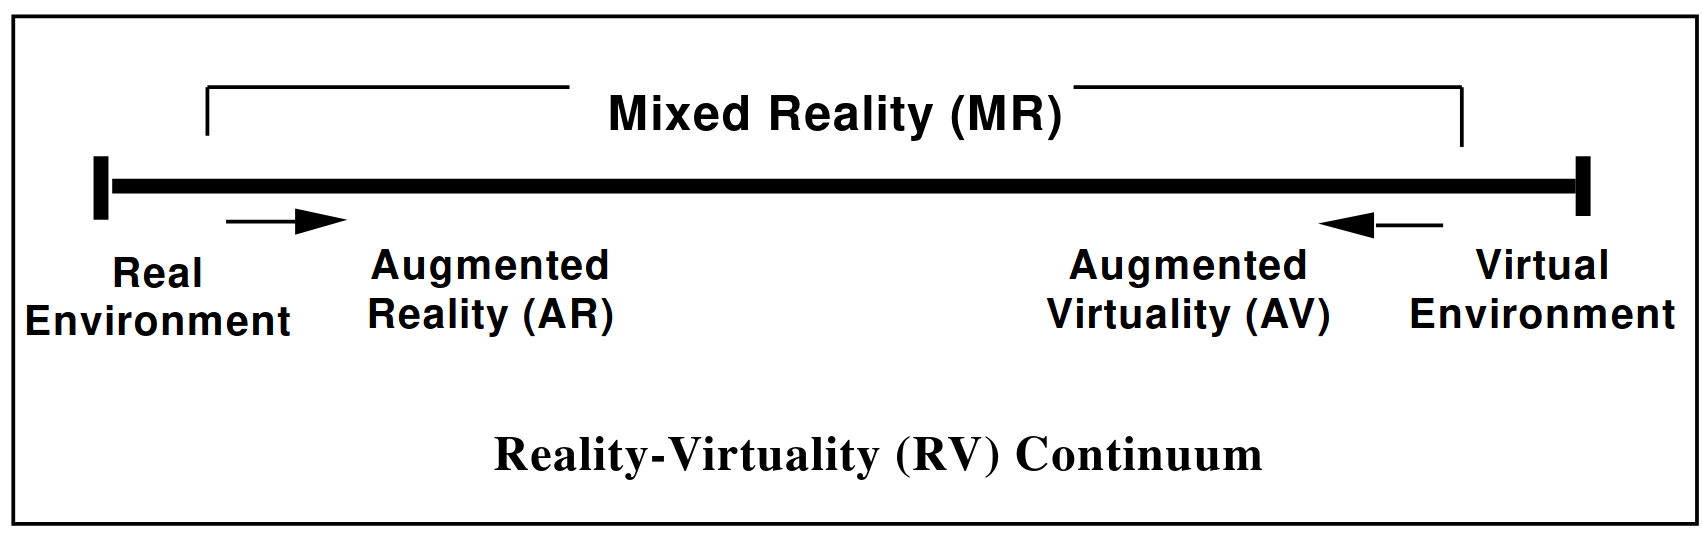
\includegraphics[width=12cm]{img/continuum.png}
  \caption{Zjednodušená reprezentácia RV kontinua \cite{milgramAugmentedRealityClass1995}.}
  \label{rv-continuum}
\end{figure}	

\subsubsection{Synonym}
V mnohých článkoch, ktoré autori \cite{speicherWhatMixedReality2019a} skúmali, sa používalo \acrshort{mr} ako synonymum pre \acrshort{ar}. To znamená, že tieto pojmy sa 
navzájom zamieňali; \acrshort{mr} bolo použité na označenie systému, ktorý jednoznačne spadal pod \acrshort{ar}, alebo bola použitá definícia \acrshort{ar} na popísanie toho,
čo niektorí autori skúmaných článkov chápali pod pojmom \acrshort{mr}.

\subsubsection{Collaboration}
Ďalší pohľad vníma \acrshort{mr} ako druh spolupráce. V tomto prípade \acrshort{mr} predstavuje interakciu medzi rôznymi používateľmi \acrshort{ar} a \acrshort{vr}, ktorí
sa nemusia spoločne nachádzať v jednom priestore. Súčasťou tohto typu \acrshort{mr} je rekonštrukcia prostredia, v ktorom sa nachádza používateľ \acrshort{ar}, pre druhého
používateľa prostredníctvom \acrshort{vr}.

\subsubsection{Combination}
V tomto prípade je \acrshort{mr} chápané ako kombinácia \acrshort{ar} a \acrshort{vr} v zmysle systému, ktorý využíva oddelené časti postavené na \acrshort{vr}, respektíve
\acrshort{ar}. Hoci tieto časti medzi sebou dokážu interagovať, nie sú navzájom pevne prepojené; systém prípadne dokáže podľa potreby prepínať medzi \acrshort{ar} a
\acrshort{vr}. Autori \cite{speicherWhatMixedReality2019a} uvádzajú ako príklad aplikáciu Pokémon GO, kde samotné chytanie Pokémonov je realizované v \acrshort{ar}, zatiaľ čo 
prehľad mapy je plne virtuálny.

\subsubsection{Alignment}
\acrshort{mr} ako zarovnanie prostredí\footnote{z angl. \emph{alignment of environments}, súosovosť} predstavuje synchronizáciu medzi skutočným a virtuálnym prostredím.
Takýto systém kombinuje virtuálne a skutočné prvky, vďaka čomu tu nájdeme čiastočný prienik s \emph{Combination}, ale prostredia samotné nemusia nutne byť \acrshort{ar}
a \acrshort{vr}. Podobnosť jestvuje aj s \emph{Collaboration}, ale bez prítomnosti aspektu spolupráce a bez toho, aby boli prostredia fyzicky oddelené. Ako príklad sa 
uvádza systém prenášajúci pohyb človeka v reálnom svete do plne imerzívneho virtuálneho prostredia prostredníctvom zariadenia Leap Motion Controller.

\subsubsection{Strong \acrshort{ar}}
Posledný pohľad na túto problematiku chápe \acrshort{mr} ako \emph{silnejšiu} verziu \acrshort{ar}. Zmiešaná realita je tu charakterizovaná pokročilým vnímaním prostredia
a pokročilými interakciami medzi používateľom a virtuálnymi objektmi, ako aj medzi virtuálnymi objektmi a prostredím. To vytvára predpoklad, že \acrshort{mr} závisí
na konkrétnom hardvéri alebo zariadení, ktoré dokáže poskytnúť požadovanú funkcionalitu. Taktiež sa predpokladá, že \emph{obyčajné} \acrshort{ar} nemá takéto schopnosti,
a tým pádom je \acrshort{mr} evolúciou \acrshort{ar}. \\\\
\noindent
Brigham uvádza, že zmiešaná realita umožňuje používateľovi vidieť reálny, fyzický svet a predmety spoločne s umelými predmetmi, ktoré sú uveriteľné a responzívne. Je to snaha o spojenie
toho najlepšieho z virtuálnej a rozšírenej reality. To, čo odlišuje zmiešanú realitu od rozšírenej, je umožnenie vnímania hĺbky a perspektívy; keď sa používateľ v zmiešanej
realite vzdiali od nejakého predmetu, tento predmet sa bude javiť menší \cite{brighamRealityCheckBasics2017}.

Medzi zariadenia, ktoré sprostredkúvajú zmiešanú realitu, patrí aj Microsoft HoloLens 2, ktorého použitie je predmetom tejto práce.
%\newpage
\subsection{Microsoft HoloLens 2}
Microsoft HoloLens 2 je \acrshort{mr} zariadenie, ktoré dokáže fungovať samostatne, bez potreby pripojenia k počítaču. Je to druhá generácia tohto zariadenia spoločnosti 
Microsoft a ponúka niekoľko zlepšení a zdokonalení oproti svomu predchodcovi. Je postavený na platforme Snapdragon 850 od spoločnosti Qualcomm, ktorá je dostatočne
výkonná na to, aby na HoloLense dokázal bežať samostatný operačný systém. Microsoft pre tento headset vytvoril upravenú verziu ich operačného systému Windows 10 pod
názvom Windows Holographic OS. 

\begin{figure}[!htbp]
  \centering
  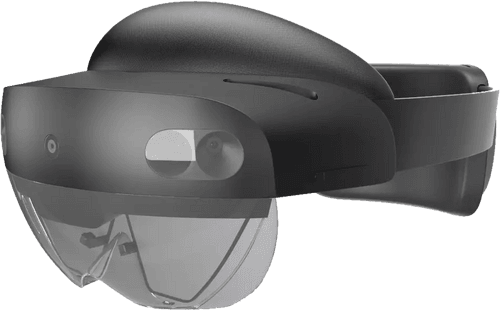
\includegraphics[width=10cm]{img/microsofthololens2.png}
  \caption{Headset Microsoft HoloLens 2.}
  \label{hololens}
\end{figure}	

%\subsubsection{Zobrazovacia technológia}
HoloLens 2 využíva na zobrazovanie obrazu dva priehľadné holografické displeje typu \acrshort{lbs}, každý s rozlíšením 1440x936 pixelov a obnovovaciou frekvenciou
 60 Hz \cite{MicrosoftHoloLensFull}. 
\acrshort{lbs} dokáže poskytnúť široké zorné pole; v spojení s vysokým rozlíšením umožňuje v prostredí používateľa zobraziť hologramy s vysokou úrovňou detailov.

Súčasťou HoloLensu sú taktiež rôzne senzory a kamery, ktoré umožňujú snímať a vyhodnocovať prostredie, v ktorom sa používateľ práve nachádza \cite{AdvancingMRExperience}. 
Dáta o prostredí sú získavané pomocou nasledujúceho vybavenia:
\begin{itemize}
  \item Kamery sledujúce prostredie vo viditeľnom spektre\footnote{Visible Light Environment Tracking}
  \item Hĺbková kamera
  \item Farebná kamera
  \item Pohybové senzory
  \item Infračervené kamery
  \item Pole mikrofónov  
\end{itemize}

Štvorica kamier sledujúcich prostredie vo viditeľnom spektre snímajú obraz v škále šedej; ich obraz sa používa na sledovanie pohybu hlavy a vytváranie priestorovej mapy.
Hĺbková kamera sníma priestor v dvoch režimoch. Prvý režim sníma priestor rýchlosťou 45 snímkov za sekundu a slúži primárne na zaznamenávanie pohybu rúk; presnú vzdialenosť
dokáže detegovať približne do jedného metra. V druhom režime, ktorý je určený na priestorové mapovanie, je rýchlosť snímania v rozmedzí jeden až päť snímkov za sekundu.
V oboch režimoch však kamera dokáže poskytovať obrázky v infračervenom spektre, ktoré nie sú ovplyvnené ambientným svetlom.
\\\\
\noindent Pohybové senzory, ktoré HoloLens používa, sú nasledovné:
\begin{itemize}
  \item akcelerometer, ktorý sníma zrýchlenie na všetkých osiach,
  \item gyroskop, ktorý slúži na detekciu rotácie, a
  \item magnetometer, ktorý pomáha určiť absolútnu orientáciu.
\end{itemize}
Farebná kamera umožňuje snímať obrázky v rozlíšení 8 megapixelov, alebo natáčať video v rôznych rozlíšeniach. Medzi jej funkcie patrí automatické zaostrovanie, vyváženie bielej,
automatické nastavenie expozície a i. Pomocou tejto kamery je možné zaznamenávať \acrshort{mr} zážitok a zdieľať ho s ostatnými ľuďmi tak, ako ho vidí používateľ 
prostredníctvom funkcie Mixed Reality Capture.

Pomocou infračerevných kamier zabudovaných v headsete je možné sledovať pohyb očí používateľa. Táto funkcia umožňuje detegovať používateľov pohľad a reagovať naň, vďaka čomu 
môže byť \acrshort{mr} zážitok intenzívnejší a interakcia s virtuálnym svetom dokáže byť intuitívnejšia. 
Prostým pohľadom dokáže používateľ presúvať virtuálne objekty, posúvať čítaný text; taktiež je možné sledovať pozornosť používateľa v danom okamihu \cite{EyeTrackingHoloLens}.
Táto funkcia je oproti predchádzajúcej verzii headsetu novinkou.

Prostredníctvom poľa mikrofónov dokáže HoloLens reagovať na hlasové povely, čo v spojení so sledovaním pohybu očí umožňuje efektívne používanie headsetu aj bez použitia rúk.

%\newpage
\subsection{Vývoj aplikácií pre Microsoft HoloLens 2}
Microsoft vývojárom poskytuje \acrshort{mrtk} (\acrlong{mrtk}), čo je multiplatformová knižnica, ktorá významne urýchľuje a zjednodušuje prácu vývojárov pri tvorbe aplikácií
pre umelú realitu. Prostredníctvom tejto knižnice je možné rýchle prototypovanie aplikácií za použitia rôznych \acrshort{ui}/\acrshort{ux} nástrojov, predpripravených šablón 
objektov (napr. tlačidiel) a hotových príkladov aplikácií \cite{valoremreplyWaysMicrosoftMixed}. Kód slúžiaci na interakciu s objektami, prostredím a senzormi headsetu
je písaný v jazyku C\#.

\acrshort{mrtk} je dostupný pre populárny herný engine Unity. Unity je dostupné bezplatne pre osobné použitie, čo robí takýto vývoj prístupný širokému spektru záujemcov.
Ďalšou možnosťou je použitie Unreal Engine, pre ktorý existuje samostatná verzia \acrshort{mrtk}.

Okrem HoloLens 2 je podporovaných niekoľko ďalších zariadení, napr. Meta Quest \cite{microsoftWhatMixedReality}. Takztiež sú podporované platformy postavené na platforme
iOS a Android. Jednou z výhod multiplatformovosti je aj jednoduchý prenos aplikácie napísanej pre pôvodnu verziu HoloLens na verziu 2. Rovnako sa dá veľká časť programu
otestovať na jednom zariadení, a na ostatných zariadeniach, s ktorými sa pri vývoji počíta, sa už len dolaďujú špecifické detaily.

Na to, aby dokázal vývojár otestovať svoju aplikáciu, nemusí mať prístup k headsetu ako takému. Nástroj s názvom HoloLens Emulator umožňuje odskúšanie takejto aplikácie 
na počítači, pričom vstupy sú simulované pomocou myši, klávesnice, prípadne ovládača Xbox. Pre použitie v emulátore nie je nutné aplikáciu žiadnym spôsobom upravovať. 
Pohyb v priestore je ovládaný rovnako, ako v typickej počítačovej hre (klávesy W, A, S a D), pohybom myši sa simuluje pohyb rúk a hlavy \cite{microsoftUsingHoloLensEmulator}.



